% THIS IS SIGPROC-SP.TEX - VERSION 3.1
% WORKS WITH V3.2SP OF ACM_PROC_ARTICLE-SP.CLS
% APRIL 2009
%
% It is an example file showing how to use the 'acm_proc_article-sp.cls' V3.2SP
% LaTeX2e document class file for Conference Proceedings submissions.
% ----------------------------------------------------------------------------------------------------------------
% This .tex file (and associated .cls V3.2SP) *DOES NOT* produce:
%       1) The Permission Statement
%       2) The Conference (location) Info information
%       3) The Copyright Line with ACM data
%       4) Page numbering
% ---------------------------------------------------------------------------------------------------------------
% It is an example which *does* use the .bib file (from which the .bbl file
% is produced).
% REMEMBER HOWEVER: After having produced the .bbl file,
% and prior to final submission,
% you need to 'insert'  your .bbl file into your source .tex file so as to provide
% ONE 'self-contained' source file.
%
% Questions regarding SIGS should be sent to
% Adrienne Griscti ---> griscti@acm.org
%
% Questions/suggestions regarding the guidelines, .tex and .cls files, etc. to
% Gerald Murray ---> murray@hq.acm.org
%
% For tracking purposes - this is V3.1SP - APRIL 2009

\documentclass{acm_proc_article-sp}
\usepackage{filecontents}

\begin{document}

\title{Analysis of Current Approaches in Topic Modeling for Twitter Data}

\numberofauthors{2} 
\author{
\alignauthor
Brian Gillespie\\
       \affaddr{Northeastern University}\\
       \affaddr{Seattle, WA}\\
       \email{bng1290@gmail.com}
\alignauthor
Shailly Saxena\\
       \affaddr{Northeastern University}\\
       \affaddr{Seattle, WA}\\
       \email{saxena.sha@husky.neu.edu}
}

\date{26 March 2016}


\maketitle
\begin{abstract}
\hspace*{5mm}Twitter is a dynamic source of text data, reflecting the changing world and how it is viewed by those who in inhabit it. Proper analysis of this data can yield very interesting insights into public opinion and the popular sentiment towards events as they unfold in real time. The ability to see which events matter to people as they emerge is highly desirable, however topic modeling of Twitter data remains somewhat elusive due to the nature of Tweets themselves. Non-standard vocabulary, limited character length, and the wide variety of tweet content often make it difficult to extract meaningful, generalized topics from the data. \\
\hspace*{5mm}In this paper, we investigate two of the more recent approaches to topic modeling of Twitter data, and compare their effectiveness against a basic TF-IDF model of raw Tweets as a base reference. In the first approach, user profiles are generated by aggregating Tweets per user. This aims to leverage the consistency of each user's Tweets, thus increasing the relevance of words within each topic. The second method attempts to modify Latent Dirichlet Allocation (LDA) such that the distribution of topics for each user is considered alongside the distribution of topics for the entire Twitter dataset. Brief results summary here. 
\end{abstract}

\keywords{Twitter, LDA, topic modeling, NLP, TF-IDF, social media} 

\section{Introduction}
\hspace*{5mm}Twitter is an excellent medium for the development of hot topics, and these topics often gain a lot of momentum as they pan out to reach a wider variety of people. Analysis of these trending topics as they develop and impact users around the world is a popular area of research in text analysis. Many times, Twitter has been a nexus for people from all over to come together and offer sympathies during tragic events such as the terrorist attacks in Brussels. Users often rally behind simple messages, and weigh in their opinions, popular or unpopular, facilitating global discourse on a brand new scale. As a whole, the variety of information contained within Twitter is loaded with the random musings of over 305 million active users. This is a great obstacle that must be overcome in order to make any generalizations about the data. The ability to distill essential topics is very desirable, as businesses strive to cater their products to an increasingly diverse and dynamic consumer base. Such knowledge can also assist with attracting new markets, and to gain a better understanding of how current markets are responding to new campaigns or product lines.\\
\hspace*{5mm}There has been much research in the structure and dynamics of microblogging networks, and many insights have been gained by looking into how users interact with one another and with the world. Attempts to glean detailed information from the actual contents of the networks however, has met with limited success. Recent developments in topic-modeling approaches to Twitter data such as Hong and Davison\cite{hong2010empirical} and Zhao, Wayne Xin, et al.\cite{zhao2011comparing} have further refined traditional topic-modeling techniques so that they better cater to the specific structure of Twitter data. In this paper, we explore some of the more promising approaches to topic modeling in tweets, and investigate their implications to further research into developing a more successful Twitter topic model.\\
\hspace*{5mm}In \cite{hong2010empirical}, various preprocessing methods were employed to increase the accuracy of Latent Dirichlet Allocation(LDA) applied to a series of tweets from the first and second weeks of November 2009. Tweets were aggregated by the User IDs of their authors, and a new set of documents was created where each document is a \textit{user profile} of a unique user id and his or her combined set of tweets. Hong and Davison saw a significant improvement in the Precision, Recall, and F1 scores of their topic models for the user profile approach, however the other alternative approaches employed did not appear to improve these same metrics as significantly. Due to the success of the \textit{user profile} approach, we will employ and evaluate this method, to further investigate its effectiveness.\\
\hspace*{5mm}In \cite{zhao2011comparing}, researchers attempted to modify LDA so as to adapt the algorithm to model Twitter data more closely. By not only considering the distribution of total topics in the data, topics were also drawn for each user, based on the understanding that each user's set of interests are relevant to how their tweets are composed.

\section{Dataset and Preprocessing}
\hspace*{5mm}The datasets used were obtained from Cheng, Caverlee, and Lee \cite{cheng2010content}. In order to reduce noise in the text data, a set of stop words were removed from the tweet bodies, the remaining words were then stemmed, and any hyperlinks were also removed. A bag of words model was created, and TF-IDF vectors were generated. For the \textit{user profile} LDA approach \cite{hong2010empirical} and the Twitter-LDA model \cite{zhao2011comparing}, the vectors were aggregated based on user IDs. We also processed each tweet for the documents ``as-is'' for the Twitter-LDA model. The training and tests datasets were merged, and then re-partitioned to prepare for 10-fold cross-validation.

\subsection{The Dataset}
\hspace*{5mm}The training dataset from Cheng, Caverlee, and Lee \cite{cheng2010content}, contains 3,844,612 tweets from 115,886 Twitter users over the time period of September 2009 to January 2010. The test set, also from \cite{cheng2010content}, contains 5,156,047 tweets from 5,136 Twitter users over the same time period. Each line of the dataset contains a unique user ID and tweet ID, text content, and a timestamp. The text content of each tweet is limited to 140 characters, and can contain references to other users of the form @username, as well as popular \#hashtags. Many tweets also include hyperlinks which are often passed through URL shorteners (e.g. http://goo.gl/uLLAe). The implications of these more anomalous text instances are considered in the next section.\\
\hspace*{5mm}An additional document corpus was generated from each dataset by aggregating tweets by user ID. This reduction is referred to as the \textit{user profile} model \cite{hong2010empirical}. After aggregation, the corpus contained a total of <115,886> documents. The largest \textit{user profile} contained (after preprocessing) <NUMBER> tokens, and the smallest contained <NUMBER> tokens. To further reduce the data, any profile containing <THRESHOLD> words was removed. After Term Frequency hashing was applied, words occurring less than <NUMBER> times were removed and more than <NUMBER> were removed\cite{cheng2010content}.
 
\subsection{Data Preprocessing and Reduction}
\hspace*{5mm}Due to the unconventional vocabulary in tweets and the large amount of noise inherent in such a diverse set of text, we decided to perform several data reduction steps. A regular expression was used to remove any odd characters and any URL links, to reduce noise in the data. After pruning the tweet contents, the text was tokenized, stop words were removed, and the remaining tokens were stemmed using the Porter Stemming library from the Natural Language Toolkit (NLTK). The prepared corpus of tweets was then converted to a set of Term Frequency (TF) vectors, using the corpora library from gensim. Gensim also provided a map of words to their hashed keys so that the LDA results could be interpreted.

\section{Model and Evaluation}
\hspace*{5mm}Latent Dirichlet Allocation, first proposed by Blei, Ng, and Jordan \cite{blei2003latent} is a generative probabilistic model, that seeks to generate mixtures of topics drawn from some distribution of topic probabilities. Each word appearing in these topics is itself probabilistically drawn from some mixture of these topics. This multilevel approach to topic generation has met with significant success in the analysis of text data, and is the subject of focused study in data mining of microblogs such as Twitter and Facebook.\\
\hspace*{5mm}When measuring the effectiveness of an LDA model, it is important to distinguish a set of metrics which give a complete picture of a word's sensibility with respect to its topic and the document corpus as a whole. To meet this need, our evaluation focuses on Precision and Recall. Additionally, we conflate these two metrics together to generate F1 scores. These metrics were performed on each modeling approach taken, and the results are detailed in the Results and Discussion section.
\subsection{LDA as a Topic Model}
\hspace*{5mm}Talk about the why and how of LDA. Then maybe a brief intro into the math, throw in a figure from the paper maybe?
\begin{figure}[h]
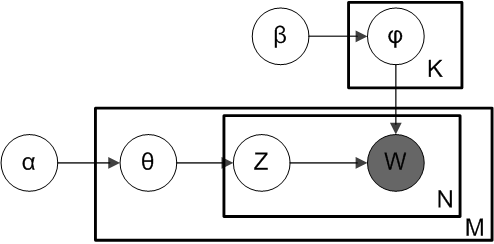
\includegraphics[scale=0.47]{figs/Smoothed_LDA}
\caption{Plate Diagram of LDA.}
\end{figure}
\subsection{Model Evaluation Metrics}
\hspace*{5mm}In order to evaluate the success of these topic modeling approaches, we decided to measure the Precision, Recall and F1 scores of the results \cite{hong2010empirical}. 
\[ \textbf{Precision = }\frac{\textbf{number of true false positives}}{\textbf{number of true positives } \mathsf{+} \textbf{ false positives }} \]
\[ \textbf{Recall = }\frac{\textbf{number of true false positives}}{\textbf{number of true positives } \mathsf{+} \textbf{ false negatives }} \]
\[ \textbf{F1 = }\frac{\textbf{Precision } \mathsf{x} \textbf{ Recall}}{\textbf{Precision } \mathsf{+} \textbf{ Recall}} \]


\begin{filecontents}{jobname.bib}
@incollection{zhao2011comparing,
	title={Comparing twitter and traditional media using topic models},
	author={Zhao, Wayne Xin and Jiang, Jing and Weng, Jianshu and He, Jing and Lim, Ee-Peng and Yan, Hongfei and Li, Xiaoming},
	booktitle={Advances in Information Retrieval},
	pages={338--349},
	year={2011},
	publisher={Springer}
}
@inproceedings{hong2010empirical,
	title={Empirical study of topic modeling in twitter},
	author={Hong, Liangjie and Davison, Brian D},
	booktitle={Proceedings of the first workshop on social media analytics},
	pages={80--88},
	year={2010},
	organization={ACM}
}
@inproceedings{cheng2010content,
	title={You Are Where You Tweet: A Content-Based Approach to Geo-locating Twitter Users},
	author={Z. Cheng, J. Caverlee, and K. Lee},
	booktitle={Proceeding of the 19th ACM Conference on Information and Knowledge Management (CIKM)},
	month={October},
	year={2010}
}
@article{blei2003latent,
	title={Latent dirichlet allocation},
	author={Blei, David M and Ng, Andrew Y and Jordan, Michael I},
	journal={the Journal of machine Learning research},
	volume={3},
	pages={993--1022},
	year={2003},
	publisher={JMLR. org}
}
\end{filecontents}

\nocite{*}

\bibliographystyle{abbrv}
\bibliography{jobname}

%\balancecolumns 

\end{document}